\section{研究方法、技术路线、实验方案}
\subsection{研究方法}
\begin{frame}{\insertsubsection——常见方法}
	\begin{columns}
		\column{0.35\textwidth}
		常见的研究方法:
		\begin{itemize}
			\item<1-> 植物多样性梯度
			\item<2-> 土壤微生物多样性梯度
			\item<3-> 演替梯度
			\item<4-> 环境因子梯度
			\item<5-> 功能群移除			
		\end{itemize}
		\column{0.65\textwidth}
		\begin{center}
			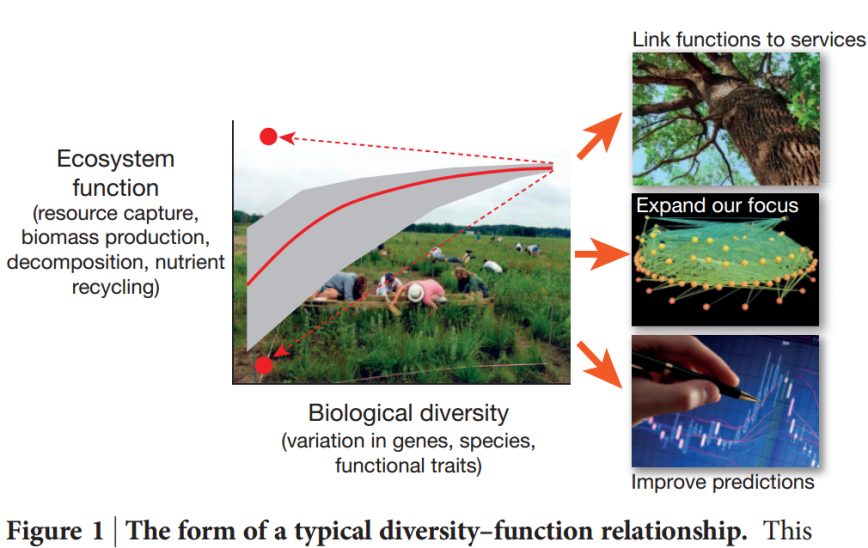
\includegraphics[width = \textwidth]{./pic/2.1.1.png}
		\end{center}
	\end{columns}
\end{frame}
\begin{frame}{\insertsubsection——研究地点}
	\begin{center}
		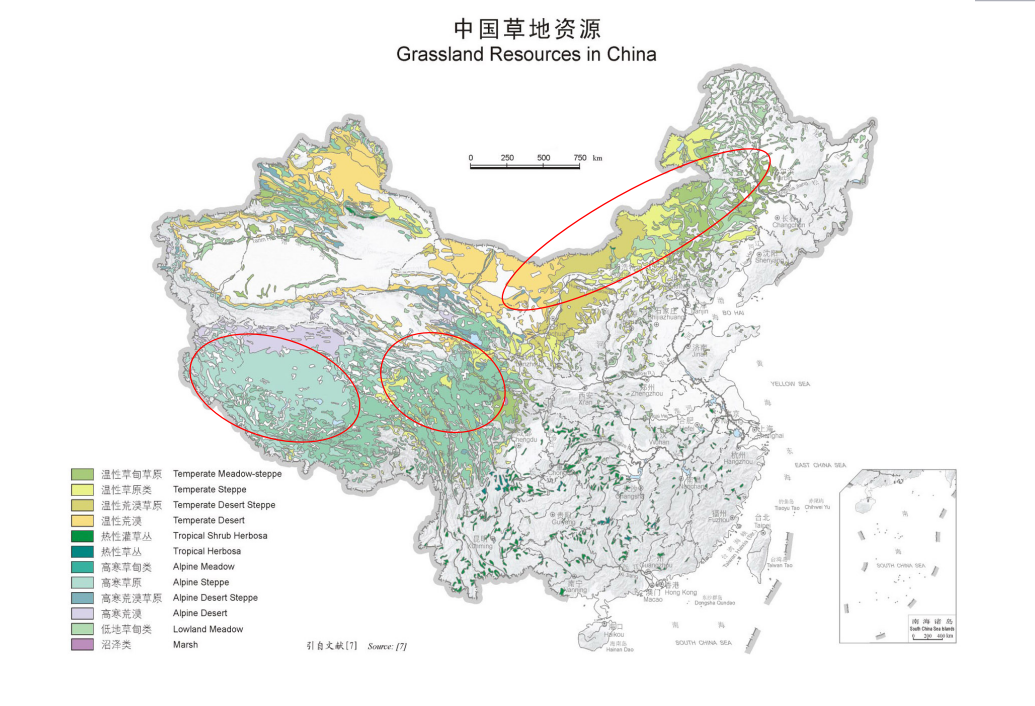
\includegraphics[width = 0.9\textwidth]{./pic/2.1.2.png}
	\end{center}
	研究地点:
	
	西藏、青海、内蒙古南北两条平行样带
\end{frame}
\begin{frame}{\insertsubsection——土壤理化性质参数}	
	
	把样带采集的土壤过筛(1mm×1mm)除去根,置于背光条件下自然风干备用。
	\vskip 2em
	1)TOC;2)TN;
	3)TP;4)MBC;
	5)MBN;\\
	6)NH4-N;7)NO3-N;8)有效P;
	9)pH
\end{frame}
\begin{frame}{\insertsubsection——植物多样性参数}
	
	$\alpha$多样性:丰富度指数(Richness), Shannon-Winer多样性指数($H'$)
	\begin{equation}\label{f_1}
	H'=-\sum_{i=1}^{S}P_i lnP_i
	\end{equation}	
	式(\ref{f_1})中$S$为物种数,$P_i$为第$i$种个体所占总个体数的比例。
\end{frame}
\begin{frame}{\insertsubsection——植物多样性参数}	
	$\beta$多样性:Bray-Curtis指数:
	\begin{equation}\label{f_2}
	 CI=\frac{2jI}{aI+bI}
	\end{equation}	
	式(\ref{f_2})中,$jI$为样地$A(jI a)$和样地$B(jI b)$共有种物种重要值较小者之和;	
	\begin{equation}\label{f_3}
	jI=\sum min(jIa+jIb)
	\end{equation}
\end{frame}
\begin{frame}{\insertsubsection——室内试验}
	
	
		\begin{center}
			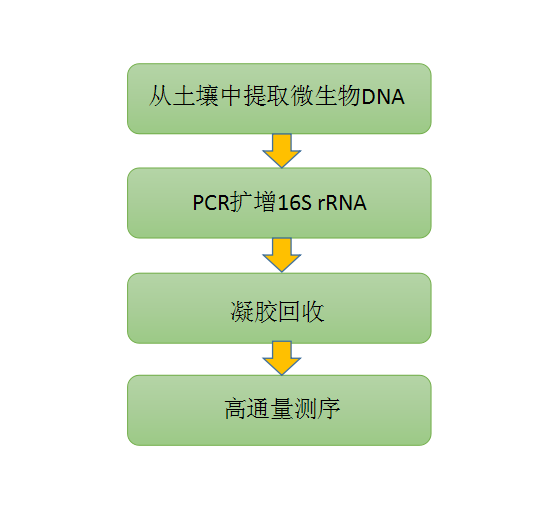
\includegraphics[width = 0.6\textwidth]{./pic/2.1.3.png}
		\end{center}
\end{frame}


\subsection{技术路线}
\begin{frame}{\insertsubsection}
	\begin{center}
		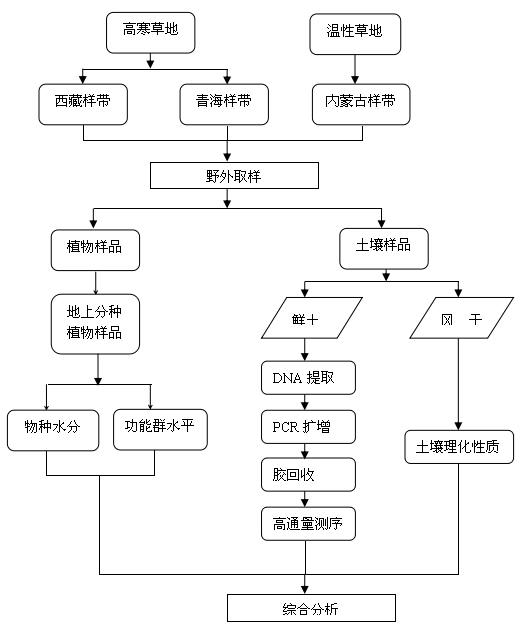
\includegraphics[width = 0.6\textwidth]{./pic/技术路线.jpg}
	\end{center}
\end{frame}
\subsection{实验方案}
\begin{frame}{\insertsubsection}
	\begin{center}
		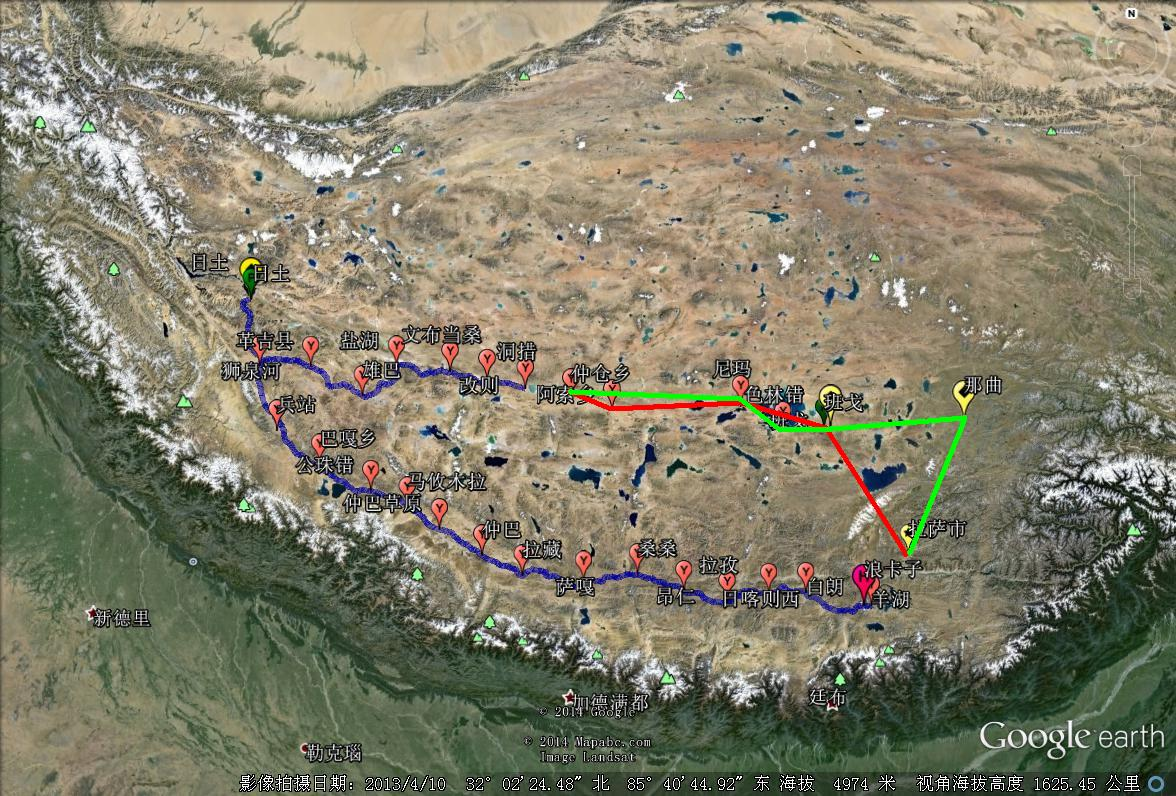
\includegraphics[width = 0.9\textwidth]{./pic/西藏瓦岗.jpg}
	\end{center}
	1)在西藏冈底斯山脉南北两侧,沿水分梯度各由东往西定点取样;
\end{frame}

\begin{frame}{\insertsubsection}	
	\begin{columns}
		\column{0.5\textwidth}
		\begin{center}
			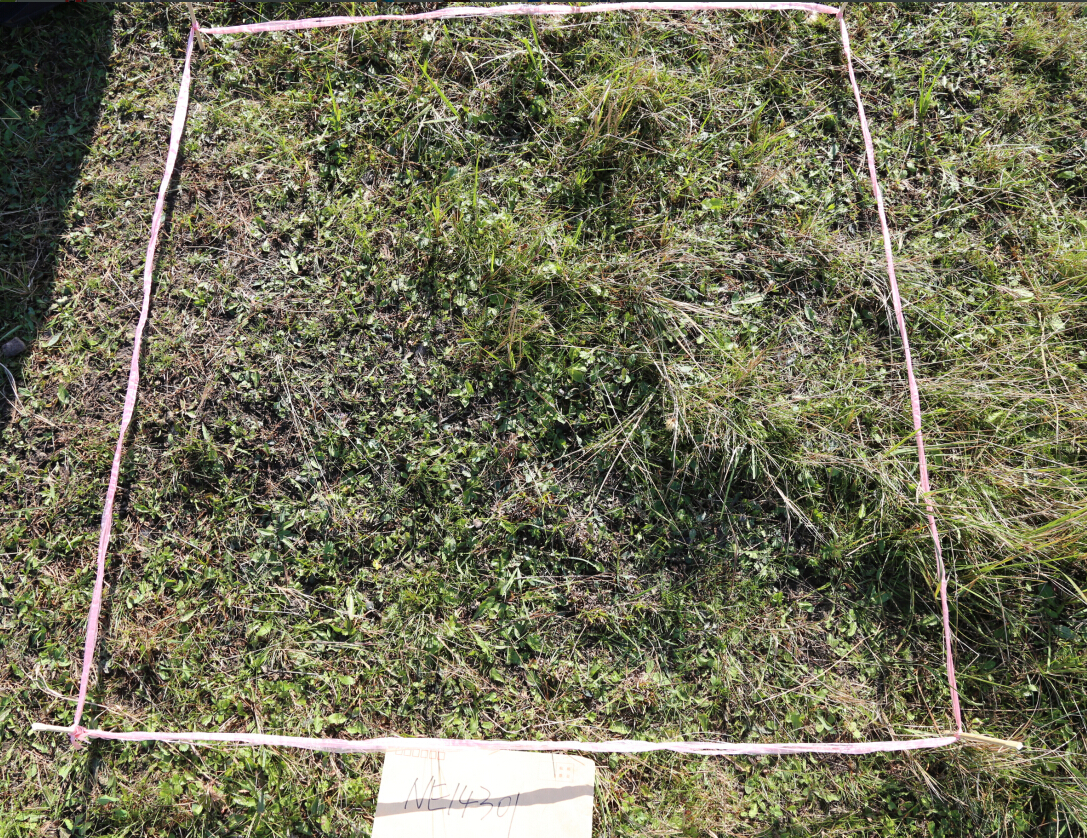
\includegraphics[width = 1.1\textwidth]{./pic/2.3.1.jpg}
		\end{center}		
		\column{0.5\textwidth}
		\begin{center}
			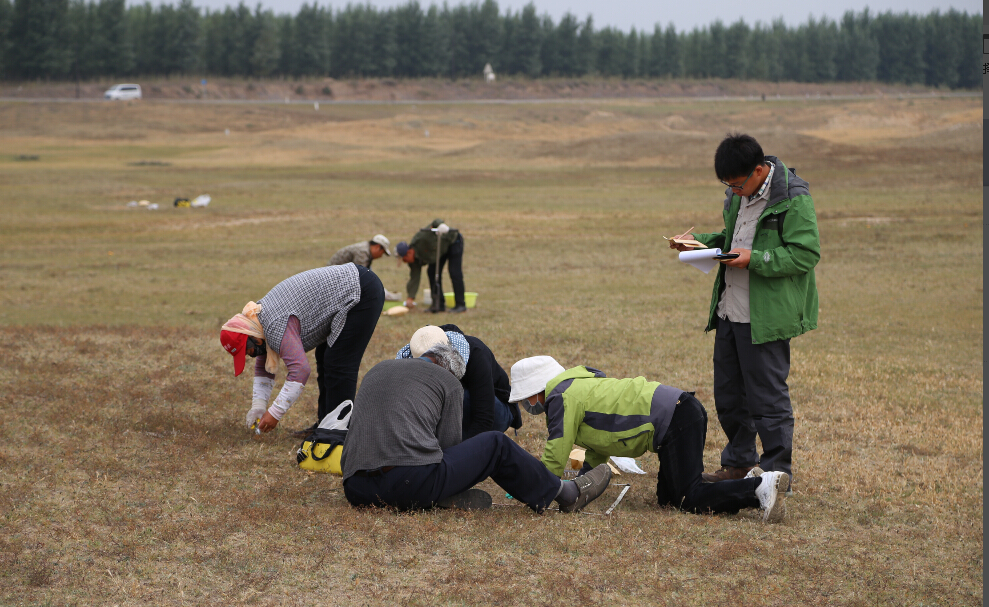
\includegraphics[width = 1.4\textwidth]{./pic/2.3.2.jpg}
		\end{center}
	\end{columns}
	\vskip 2em
	2)在每个取样点,随机选择5个1m×1m的样方,记录每个物种(随机选取5株)的高度,分种剪取地上植物生物量,称鲜重,实验室65℃烘72小时,称干重;	
\end{frame}
\begin{frame}{\insertsubsection}	
	\begin{columns}
		\column{0.5\textwidth}
		\begin{center}
			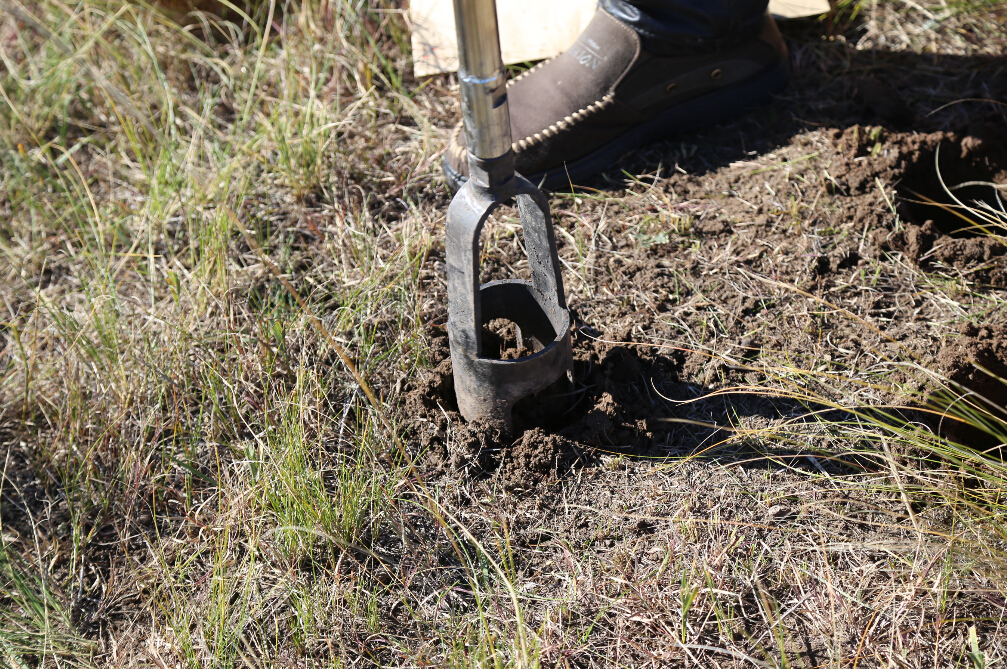
\includegraphics[width = 1.1\textwidth]{./pic/2.3.3.jpg}
		\end{center}		
		\column{0.5\textwidth}	
		\begin{center}
			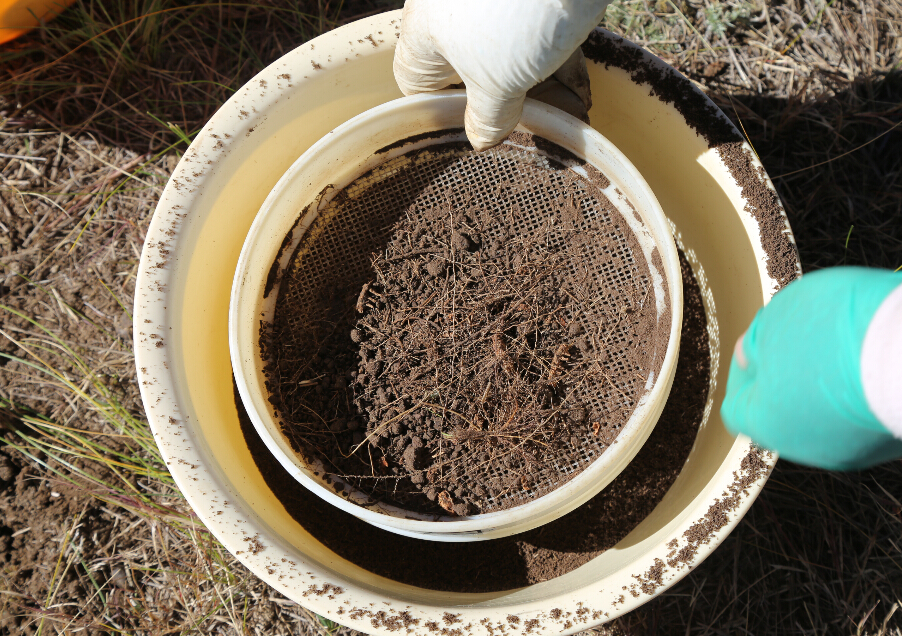
\includegraphics[width = 1.05\textwidth]{./pic/2.3.4.jpg}
		\end{center}
	\end{columns}
	\vskip 2em
	3)在每个取样点随即选择的5个1m×1m的样方剪除地上生物量后,用5cm根钻每层(0-10cm、10-20cm、20-30cm)取3钻土壤样品并均匀混合,一半土壤样品迅速放入野外冰箱并冷冻保存,用于提取微生物DNA;另外一半带回实验室风干,用于测量土壤的理化性质;	
\end{frame}

\begin{frame}{\insertsubsection}
\begin{center}
	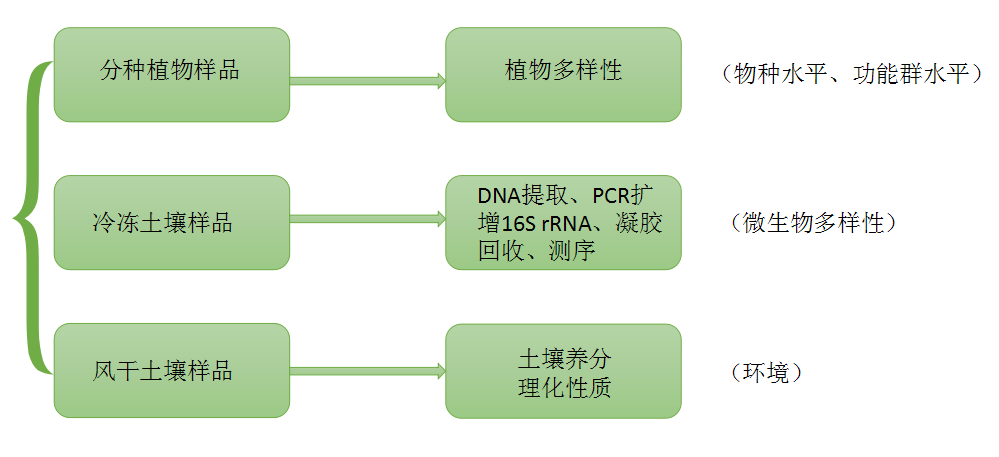
\includegraphics[width =\textwidth]{./pic/2.3.5.png}
\end{center}
\end{frame}


